\documentclass{report}
\usepackage{graphicx}
\usepackage{amsmath}
\usepackage{rotating}
\usepackage{appendix}
\usepackage{mathtools}
\setlength{\parskip}{1em}
\renewcommand{\abstractname}{Summary}
\usepackage{nomencl}
\usepackage{multirow}
\usepackage{placeins}
\makenomenclature

\begin{document}
\begin{titlepage}
	\centering
	
\includegraphics[width=0.25\textwidth]{graphics/logo}\par\vspace{1cm}
	{\scshape\LARGE University of Bath \par}
	\vspace{1cm}
	{\scshape\Large FINAL YEAR Meng PROJECT REPORT\par}
	\vspace{1cm}
	{\huge\bfseries Wave energy converter power increase through active control: Fixed Gains\par}
	\vspace{2cm}
	{\Large\itshape Carl Selig\par}

	\vfill
	
	supervised by\par
	Dr.~Andrew \textsc{Hillis}\par
	assessed by\par
	Dr.~Joseph \textsc{Flynn}

	\vfill
	
\tiny{I certify that I have read and understood the entry in the Student Handbook for the
Department of Mechanical Engineering on Cheating and Plagiarism and that all
material in this assignment is my own work, except where I have indicated with
appropriate references. Signed: ...........}

% Bottom of the page
	{\large \today\par}
\end{titlepage}
This report presents work performed in the field of Wave Power, a promising source of renewable energy. It concerns the development and investigation of a control system for a type of device known as a Wave Energy Converter. The specific device which is considered is known as WaveSub\cite{waveSub} and consists of a submerged float tethered to a platform which extracts power from passing waves.

In previous work a control strategy known as Simple and Effective control \cite{ringwood} was adapted for use with a simulated model of the WaveSub device. However, a drifting problem was observed where the device would deviate from its home position over time, exceeding the constraints of the device. If this were to happen in real life the device may be damaged.

This project methodically recreates the Simple and Effective control strategy for the device, seeking to reproduce this drifting problem. The problem was re-created. 

Methods of resolving the issue were investigated. Some evidence was found to suggest that the issue was caused by a flaw in the constraints of the Simple and Effective control strategy. An integral feedback loop was added that successfully eliminated the drifting problem in a simplistic simulation environment.

Finally the power generation of the device was compared to a passively damped, optimally tuned control strategy and found to generate more power in gentle sea-states, but less power in violent sea states. The largest percentage increase in power was 162.2\%, whilst the biggest decrease was 11.0\%.

Overall the method was found to have promise, but further research is required before recommendations on physical experimentation can be made.
\begin{abstract}

\end{abstract}
\section*{Acknowledgements}
\paragraph{I would like to thank Dr. Andrew Hillis for going above and beyond the role of supervisor.} 
\paragraph{I also wish to thank my family and friends for providing support and a significant amount of proof reading.}
\paragraph{Finally I thank my therapist, Laura Keyte, for private reasons.}
\tableofcontents
\listoffigures
\listoftables

\mbox{}

\nomenclature{$WEC$}{Wave Energy Converter}
\nomenclature{$IMC$}{Internal Model Control}
\nomenclature{$DOF$}{Degree(s) of Freedom}
\nomenclature{$SISO$}{Single Input Single Output}
\nomenclature{$MIMO$}{Multiple Input Multiple Output}
\nomenclature{$Plant$}{The physical system which is being controlled}
\nomenclature{$MATLAB$}{Matrix Laboratory. A programming language and development environment specialised for the manipulation of matrices.}
\nomenclature{$Simulink$}{A graphical programming environment based on MATLAB. Users manipulate dynamic systems by placing and connecting blocks.}

\printnomenclature

\chapter{Introduction}
Wave power refers to a group of technologies that harvest energy from sea waves. It is distinct from Tidal power. Wave power is relevant as a renewable energy source that has advantages over other sources such as solar and wind. Most notably, it constantly produces a base amount of power; can be used along most coastlines; and has a low initial expenditure. \cite{carbonTrust}

This report seeks to present the results of the research project conducted by the Author as well as the means to reproduce them. The project is part of a larger research effort to increase the power generation of Wave Energy Converters (WECs) through control system design. It is hoped that improved power generation will increase the commercial viability of the field. Wave power is already considered a viable energy source for the UK \cite{carbonTrust} but has not seen widespread commerical adoption at the time of writing \cite{europeanMarineEnergyCenter}.

There have been two WEC projects in the UK that have reached commercialisation. Pelamis from Pelamis Wave Power and Oyster from Aquamarine Systems\cite{europeanMarineEnergyCenter}. Figure \ref{previousWECs} shows these devices as they were installed. Pelamis 1 was installed in 2004 and became the first WEC to provide power to a National Grid. Pelamis 2 became the first WEC to be purchased by a utility company in 2009. Oyster was installed in 2012. Both devices provided power to the National Grid over the course of their lifetimes.

\begin{figure}
\centering
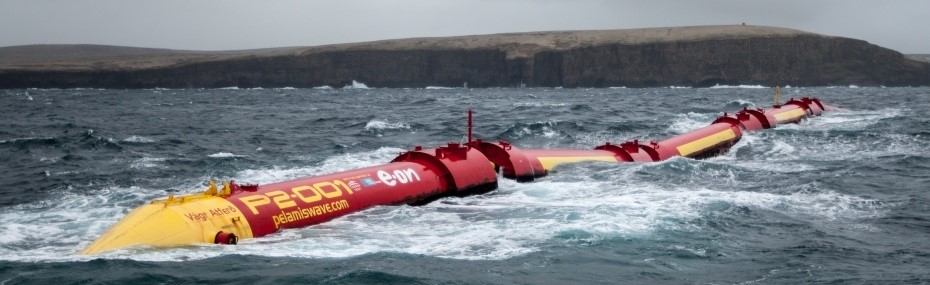
\includegraphics[height=0.2\textwidth]{graphics/pelamis}
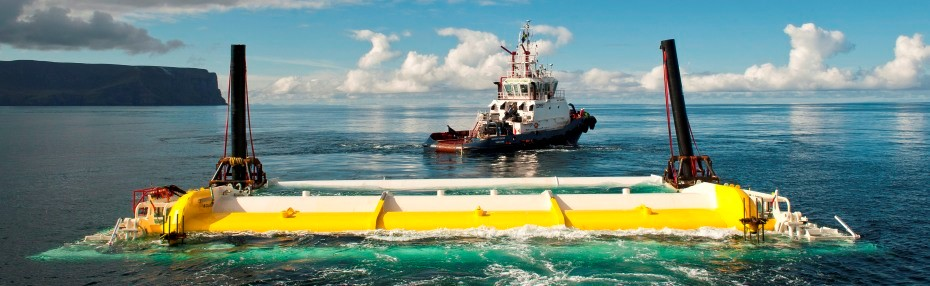
\includegraphics[height=0.2\textwidth]{graphics/oyster}
\caption{Pelamis 2 (Top) and Oyster (Bottom) as installed at the Billia Croo wave test site in Orkney, Scotland \cite{europeanMarineEnergyCenter}.}
\label{previousWECs}
\end{figure}

\FloatBarrier

According to the Carbon Trust \cite{carbonTrust} the development of a WEC with improved power generation performance and lower initial costs would positively affect the adoption of the technology in the UK.

One way of achieving these goals is to use a control system. In this project an in-development WEC known as WaveSub\cite{waveSub} is used to investigate the effectiveness of a computationally cheap control scheme that, if successful, may fulfil both requirements.

The WaveSub device consists of a submerged cylindrical float tethered to an underwater platform via 4 cables\cite{waveSub}. The cables drive Power Take Offs (PTOs) that can extract energy from the motion of the float relative to the platform \cite{waveSub}. In this project these PTOs are modelled as cable drums.

A model of the Wave Sub device has been produced in prior work by A. Hillis, the project supervisor \cite{andyMPC}. Figure \ref{fig:waveSub} shows a published graphic\cite{waveSub} of this device against the modelled WEC\cite{andyMPC}. It was chosen as a generic example of a multi-DOF WEC. The Carbon Trust describes multi-DOF WECs as being of particular interest to UK energy infrastructure due to their increased potential for energy capture over single DOF WECs \cite{carbonTrust}.

\begin{figure}
\centering
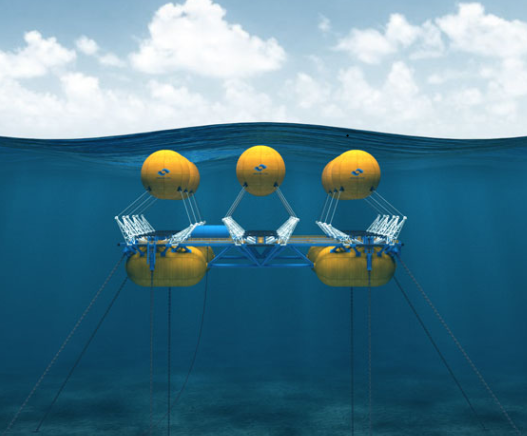
\includegraphics[height=0.4\textwidth]{graphics/waveSub}
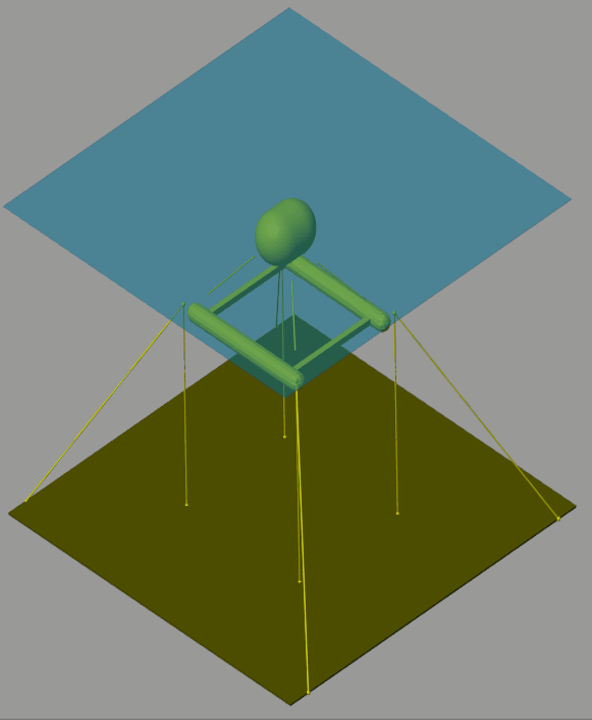
\includegraphics[height=0.4\textwidth]{graphics/wecSimFloat}
\caption{A graphic of an array of 9 WaveSub devices(left)\cite{waveSub} versus the modelled WEC(right). Note that cable arms exist in the left figure but are absent in the right due to divergent design.}
\label{fig:waveSub}
\end{figure}
\FloatBarrier

The model shown in figure \ref{fig:waveSub}  was created using a simulation environment known as wecSim\cite{wecSim} which was originally developed by a collaboration with the US department of Energy, and then adapted for use with the WaveSub device by Marine Power Systems and associates. \cite{waveSub}.

This simulation was used in prior works by Dr. Hillis to compare the power extraction of a Model Predictive Control (MPC) scheme to an, ``Optimally tuned, passively damped,'' system \cite{andyMPC}. This approach was also used in this project to assess control system performance. 

Many control schemes have been used to increase the power absorption of the WaveSub device and other WECs such as floating-point absorbers \cite{abdelkhalik2017a}\cite{abdelkhalik2018a}. Of note is a scheme known as, ``Simple and Effective'' control proposed by John Ringwood and Francesco Fusco \cite{ringwood}. They claim that this scheme approaches the effectiveness of an MPC scheme whilst being both simpler and more robust. The claim of having advantages over MPC is attractive since MPC is considered an industrial standard due to its ubiquity in digital controllers \cite{gorinevsky2005a}. MPC schemes are straightforward to implement and can optimise for the present time period whilst also considering future input. They are understood well enough that they can often be redesigned ``on the fly,'' \cite{gorinevsky2005a}. Both control schemes rely on a model of the system. In the case of Simple and Effective control the system uses an analytical model to predict Wave Excitation Force. This is taken as an input, then passed to an Extended Kalman Filter and an adaptive law based on wave peak frequency to evolve an optimal velocity trajectory. The control system then subjects the WEC PTO to Proportional-Integral control in order that the prime mover(float) tracks the velocity trajectory. The block-diagram for this scheme is reproduced below in figure \ref{ringwoodBlockDiagram}. 

\begin{figure}
\centering
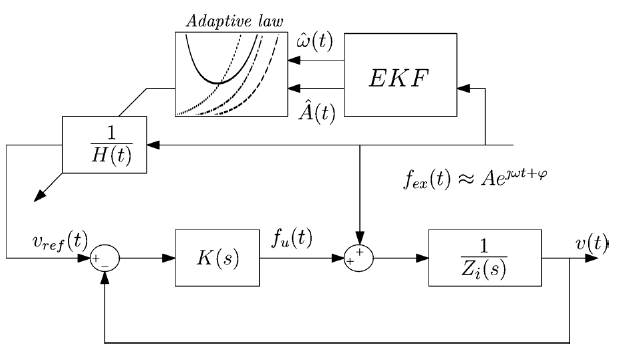
\includegraphics[height=0.4\textwidth]{graphics/ringwoodBlockDiagram}
\caption{Reproduction of figure 3 from ``A Simple and Effective Real-Time Controller for Wave Energy Converters,'' \cite{ringwood}}
\label{ringwoodBlockDiagram}
\end{figure}
\FloatBarrier

Shown are the estimated Wave Excitation Force input, $f_ex$ (t); the Extended Kalman Filter (EKF) and Adaptive law implementation. Wave Excitation Force is estimated as sinusoidal. The Simple and Effective control scheme therefore offers a significant advantage over more computationally intensive methods, including MPC. However, these results have only been shown to be true for single DOF WECs. In unpublished work, Hillis has implemented this control scheme in a 6 DOF system\cite{andyMPC}. He has observed that the float drifts from its home position over time, eventually violating the device's constraints. 

This project presents a methodical re-creation of Hillis' work, and shows that this drifting problem most likely arises due to flawed assumptions in the Simple and Effective control scheme. A potential resolution to the problem is proposed and power generation compared to a passively damped, optimally tuned system is examined.

\chapter{Literature Review}
The modern concept of wave power was first proposed in 1974 by Stephen Salter in the form of the self-styled Salter duck \cite{salterDuck}. This device was proposed as an alternative to oil during the 1973 Oil Crisis in the UK. As shown in Figure 1 the Salter duck generates power by having its vane, or beak (a) bobbed by incoming waves. This produces an oscillation which is transferred to an internal drum(h) via a ratchet(c and d). This turns the bobbing motion caused by the waves into rotary motion which can be used to generate power. Note that the water level (e) is lower behind the device as energy has been removed from the wave.

\begin{figure}
\centering
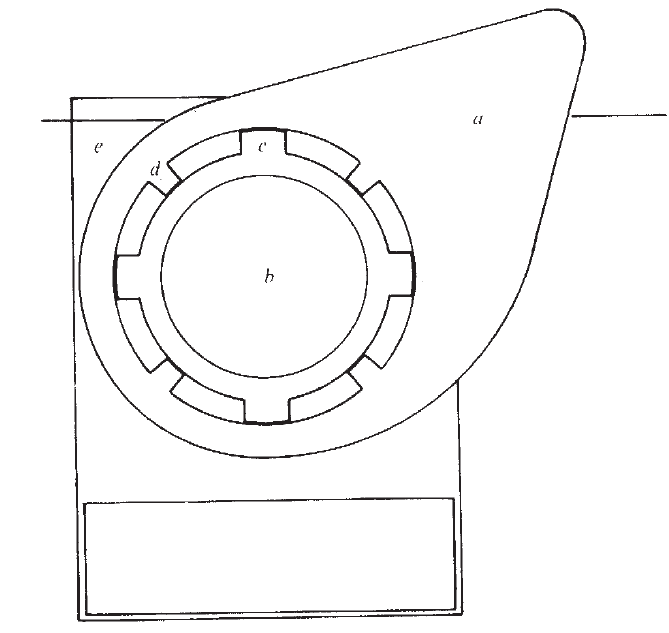
\includegraphics[scale=0.25]{graphics/duck}
\caption{A reproduction of a figure from ``Wave Power,''\cite{salterDuck}. ``a. vane; b, a hollow cylindrical member; c, paraxial ridges; d, inward facing ridges on the vane; e, vertical fin between this vane and the next.''}
\label{fig:duck}
\end{figure}

Salter is considered a foundational figure in the sector \cite{gorinevsky2005a}. So it is only fitting that the first piece of literature to be considered is his own account of his work. It is titled ``Wave Power: Nostalgic Ramblings, future hopes, and heretical suggestions'' \cite{salterRamble}.

Despite the humorous title and less than perfectly rigorous approach, this report provides a factual account of the beginnings of the field. Opinion is not always clearly stated, so care must be taken by the reader to separate the conjecture from the history. The scientific descriptions of the device, however, are clear and accurate. This makes the work a good introduction to the subject area. 

As a brief summary, Salter received funding from the UK Department of Energy to set up a laboratory in Edinburgh. Wave power then garnered interest from other British academics, notably David Evans in Bristol who invented the Bristol Cylinder \cite{evans1979a}. Evans also developed theories on the hydrodynamics and efficiency of WECs under idealised conditions \cite{evans1976a}. His work concerns a one-dimensional scenario where waves are modelled as perfect sinusoids that meet the WEC at right angles. This is not the case in nature and thus his claim that 100\% extraction of wave energy is possible has never been produced in practice.

Unfortunately, with the conclusion of the Oil Crisis, Salter and Evans found it increasingly difficult to secure funding for their research and none of their devices have been brought to market. In his report, Salter blames pressure from the nuclear sector and ``others [who] set out to destroy what they saw to be a threat,'' \cite{salterRamble}. He then goes on to explain that whilst WECs were initially billed as very simple the reality is significantly more complex.

To understand just how complex the field has become it is necessary to review works that represent the state of the art in the field. Many researchers in the field, including this projects' supervisor A. Hillis, have presented their work at the European Wave and Tidal Energy Conference (EWTEC) \cite{andyMPC}\cite{andyModelErrors}\cite{nguyen2018a}\cite{abdelkhalik2017a}. The most recent conference proceedigns have therefore been taken as source of state of the art research\cite{EWTEC}.

The proceedings are generally professional and clear. Although it appears there has been comparatively little work on multi-DOF WECs compared to more constrained devices. In general the field has become far more practical since Salter and Evans' time, with papers such as ``Wave Excitation Force Estimation for Wave Energy Converters of the Point-Absorber Type'' \cite{nguyen2018a} examining practical limitations of sensors and experimental results in detail.

There is a single piece of literature that underpins the majority of this project. It is titled ``A Simple and Effective Real-Time controller for Wave Energy Converters'' by Fusco and Ringwood \cite{ringwood}. This paper presents the Simple and Effective control strategy discussed in the Introduction. It is particularly well written, concisely providing all the information needed to reproduce the control system. This Simple and Effective control system is shown to produce near-maximal power generation in a 1 DOF WEC whilst being computationally cheap. As mentioned this is a highly desirable result \cite{carbonTrust}.

This work was previously singled out and recreated by this project's supervisor, A. Hillis. He attempted to adapt it to the WaveSub device, but discovered that the float exhibited a drift from its home position, eventually violating the physical constraints of the system. This work seeks to review this work and determine whether this drift problem is the result of Hillis' implementation, an incompatibility of the control strategy with the WaveSub Device, or a flaw in Ringwood's work.


\chapter{Aims and Objectives}
The aims of this projected are phrased as 3 research questions.
\begin{enumerate}
\item{Does a drift problem occur if Ringwood's Simple and Effective Control strategy is adapted for planar motion?}
\item{If the drift problem exists, can it be resolved?}
\item{How much power does this implementation generate compared to an optimally tuned, passively damped system?}
\end{enumerate}

To answer these questions, it was necessary to achieve the following objectives.

\begin{enumerate}
\item{Reproduce Ringwood's Simple and Effective control system for a planar model and regular sea-states.}
	\begin{enumerate}
		\item{Find a way to create an inverse of the State-Space model of the WEC}
		\item{Create an Internal Model Controller (IMC) and verify that it can make the state-space model track simple 			signals such as sine waves.}
	\end{enumerate}
\item{Adapt the control system for use with irregular sea states.}
	\begin{enumerate}
		\item{Produce look-up tables from bode plots of the radiation transfer functions.}
		\item{Implement the adaptive law of the Simple and Effective control method \cite{ringwood}.}
		\item{Implement the Extended Kalman Filter and tune it using sea-states generated by WecSim.}
		\item{Implement the position constraints using conditional Simulink logic blocks.}
	\end{enumerate}

\item{Record the Results of the Simple and Effective Control Scheme and answer research question 1.}
\item{Implement an integral feedback loop}
\item{Record the results and answer research question 2.}
\item{Tune the system and produce final results.}
\item{Answer research question 3.}
\item{Produce the Final Report}
\end{enumerate}

Previously this list included an objective to implement the controller within the WecSim environment. Unfortunately this could not be completed until the very end of the project due to the reasons discussed in section \ref{difficulties}. The results from the previous objectives were researched instead.

\chapter{Research Methodology}
This research seeks to confirm the drift result previously produced by the project supervisor, Dr. Hillis. It makes use of much of his work as a foundation but seeks to reproduce his findings using independent work. By reviewing in this way it is hoped that a greater understanding of the Simple and Effective control method as it applies to multi-DOF WECs can be reached.

\section{Positivism and Simulation}
This research makes use of a positivist approach wherein hypotheses are proposed and then either refuted or not-refuted by physical evidence. This project is also a simulation-based project, and thus does not produce physical evidence.

This contradiction is resolved by the understanding that a simulation can produce results that are representative of results in the real world. This is supported by experience with well-estabished models such as the Pierson-Moskowitz Spectrum relation\cite{OGPM} which has been extensively reviewed\cite{PMReview} and found to be representative of reality. 

Well-established models are not always available. Less well established models such as the State-Space model of the float \cite{andyMPC} are used as well as novel inventions. These cases are clearly stated and the simplifying assumptions used to produce them are catalogued in section \ref{section:assumptions}. Since the author creates both the system and its test it is possible to inadvertently bias results by disproportionately including or excluding assumptions that increase the likelihood of significant results. Whilst every effort is made to be rigorous this bias can only truly be eliminated through experimental verification.

Physical verification is not required unless a significant result has been found. For this and other practical reasons real world experimentation is outside of the scope of this project. If significant results are found then this project will serve as an inexpensive precursor to physical testing. If significant results are not found then physical testing may be applied more fruitfully elsewhere. Historically, simplifying assumptions have made significant simulation results easier to produce\cite{PMReview}. This suggests that the failure to find significant results makes a strong case that there is nothing to be found from further research.

\section{Equipment}
The only physical apparatus used in this project was the author's personal computer.

The software used to create and run the simulation was MATLAB R2018b and Simulink 9.3. The licenses for this software were obtained through the University of Bath.

Git and its associated platform Github were used to backup and distribute all project files. A link to the repository is provided in appendix \ref{github}

The typsetting environment, \LaTeX , was used to produce this report and other documents.
\chapter{Simple and Effective Control}
Simple and effective control refers to a strategy presented by Fusco and Ringwood in their paper, ``A simple and effective real-time controller for wave energy converters,''\cite{ringwood}. This strategy was designed for a 1-DOF WEC, however the WaveSub device considered in this project is a 6-DOF device. This complicates the implementation of simple and effective control. Simplifying assumptions were made which are described in Section \ref{section: assumptions}. The most important of these is the assumption that the WaveSub device behaves as a planar device, and that only surge and heave motions are controlled. Therefore the control strategy need only be adapted for 2 DOF, rather than 6.

Figure \ref{fig:fullControl} shows the full implementation of the control strategy in the Simulink environment. This chapter will detail each component in sufficient detail that the reader may re-create the system. The input to the system is a 6 element vector of wave excitation forces in each dimension($F_{ex}$). The output is 6 element vector of float velocities in the same dimensions. The 6 dimensions and their order in the vector are Surge, Sway, Heave, Roll, Pitch, and Yaw.

\begin{figure}[b]
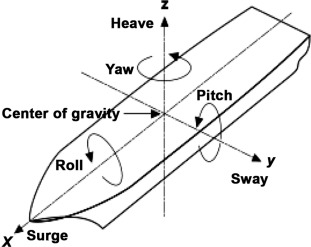
\includegraphics{graphics/dimensionsPic}
\centering
\caption{The 6 degrees of freedom relative to a boat. For the modelled float shown in figure \ref{fig:waveSub} the Yaw axis ($y$) is coincident with the cylindrical axis of the float. Figure reproduced from ``Deepwater Drilling''\cite{dimensionsPic}.}
\label{dimensionsPic}
\end{figure}

\begin{figure}[t]
\hspace{-2cm}
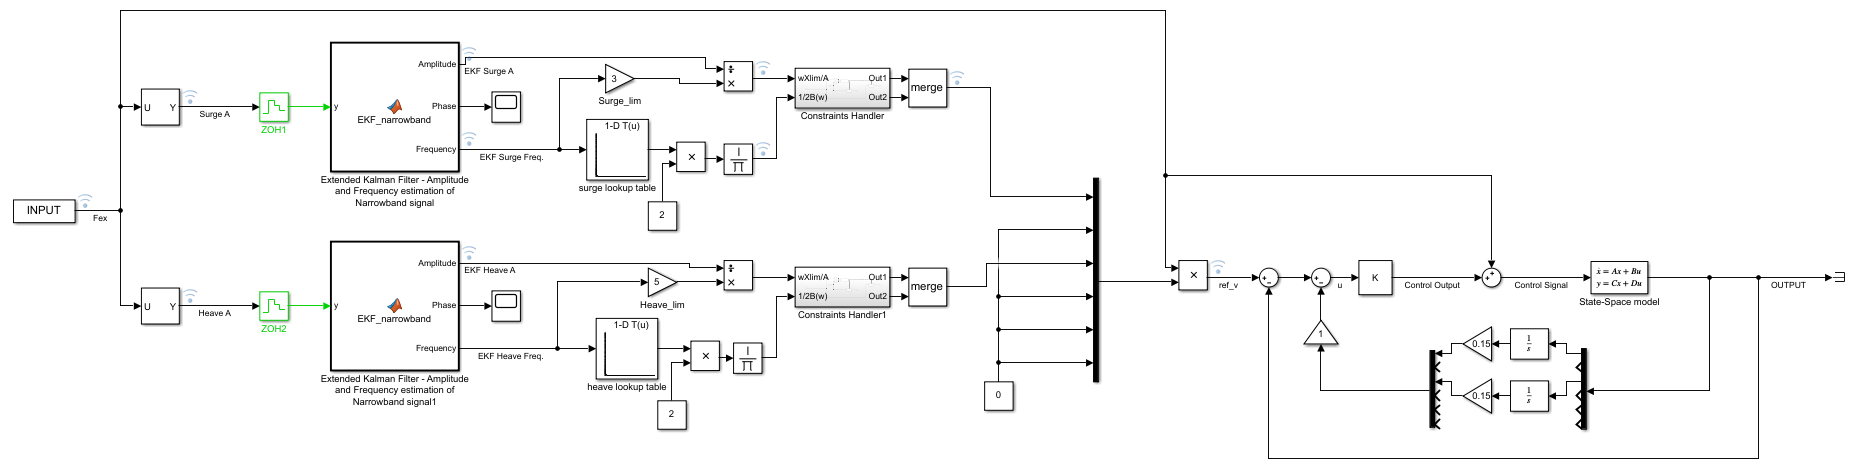
\includegraphics[scale=0.6]{graphics/fullControlSystem}
\caption{The full implementation of simple and Effective Control for the WaveSub device.}
\label{fig:fullControl}
\end{figure}

\FloatBarrier
%Fusco and Ringwood report that their control strategy provides, "levels of power capture close to MPC in most sea states... without the need of predictions and the solution of an optimization[sic] problem in real time."\cite{ringwood}. %Move this to another section.


\section{Simplifying assumptions}
\label{section:assumptions}

Sea states are modelled as irregular waves, meaning that they are the finite sum of many simple harmonic (regular) waves. Real life waves can be described perfectly as an infinite sum of regular waves, but this cannot be calculated in real-time. The waves are created from a pseudo-random combination, rather than being based on recorded data.

The energy distribution within a generated irregular wave is modelled using an empirical relationship known as the Pierson-Moskowitz spectrum. The technique is fully described in "A proposed spectral form for fully developed wind seas based on the similarity theory of S. A. Kitaigorodskii," by Pierson and Moskowitz\cite{OGPM}. This spectrum relates wave frequency and energy distribution and is based on the assumption that sea waves are in equilibrium with the wind. A 2003 review paper using modern wave data reaffirmed that "for the chosen data only... [the spectrum] provides statistically robust relations."\cite{PMReview}

It is assumed that most sea waves will be between 0.5 and 6.5 metres in significant height (Hs), and have a period between 6 and 16 seconds. Sea-state samples were created at half metre and whole second intervals in each of these ranges respectively. This is assumed to be representative of all sea states that the WEC would encounter in real life. This is based on the same study performed by Pierson and Moskowitz mentioned above \cite{OGPM}.

The float is modelled by a state-space model taken from the project supervisor's unpublished work\cite{andyMPC}. In this model it is assumed that the platform holding the PTOs is stationary. In the WECSim environment motion of the platform due to wave excitation force is modelled.

It is assumed that the signal noise that would be generated by real sensors would not significantly affect the performance of the kalman filter and hence the development of the reference velocity. This noise was not modelled in the wave excitation data.

Wave excitation force is assumed to be negligible in all dimensions save for Surge, Heave, and pitch meaning that the float dynamics can be modelled as planar. In addition, cross-terms that relate forces across dimensions are neglected.

\section{Internal Model Control}
Internal Model Control(IMC) involves creating a model of the plant, and then inverting it. The inverse model produces a  signal that will reproduce the control signal when given as input to the plant. This method is reliant on accurate modelling.

Figure \ref{fig:IMC} shows the implemented controller. It is a positive feedback loop, where the forward path is an inverse state-space model of the float, and the feedback path is the state space model. It is implemented as described in Ringwood's paper \cite{ringwood}.

\begin{figure}
\centering
\hspace{-1cm}
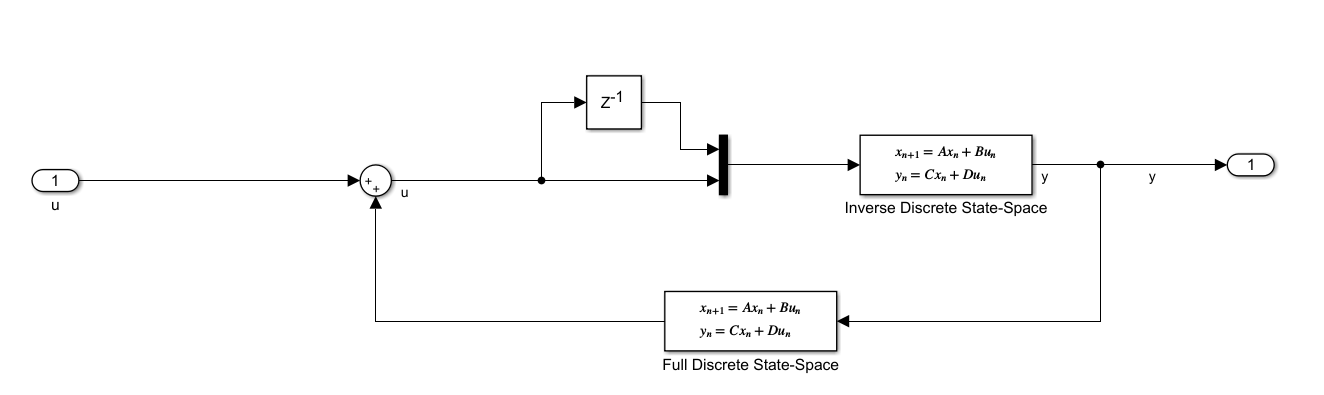
\includegraphics[scale=0.5]{graphics/IMC}
\caption{IMC implementation using an inverted state space model.}
\label{fig:IMC}
\end{figure}

The model used is a state space model taken from unpublished work by the project supervisor \cite{andyMPC}. Its derivation is outside the scope of this project. It takes 3 input forces and 3 input torques, one for each DOF. It outputs 3 velocities and 3 angular velocities. The inversion of this state space model is novel work, and is detailed in section \ref{SSInverse} The only change is that the MATLAB command, "c2d" has been used to turn the continuous-time state-space model into discrete-time. Using discrete time also forces the Simulink Solver to use a known numerical method. This prevents errors cause by mismatched solver methods.

\section{Inverting the state-space model}
\label{SSInverse}
The desired inverse will map the outputs of the state-space model to its inputs.

One inversion method is to convert the state-space system into a system of transfer functions. In this case the inverse is the reciprocal of the transfer function. This method is complicated by the fact that the plant is a 6x6 MIMO system. Generating corresponding transfer functions using inbuilt MATLAB methods results in 36 high order transfer functions.

This over-fitting of the model can be corrected by manually fitting lower order transfer functions to the system. The project supervisor has used this approach in unpublished work\cite{andyModelErrors}. The results of this work have been provided for comparison in the Results section.

Another inversion method known as the Massay-Sain algorithm has been used instead. It is able to overcome some of the shortcomings of the transfer function method. It does not require a filter to be stable; it calculates all cross terms; and does not over-fit the model.

The Massey-Sain algorithm was first presented by Sain and Massay in 1969\cite{OGMassaySain}. In 2004 it was summarised in a lecture given by Professor S. Sundaram\cite{Sundaram}. The following derivation is paraphrased from Sundaram's lecture and simplified.

First it is necessary to test whether or not the system is invertible. All discrete-time state space systems are of the form
\begin{equation}
\label{definition1}
	x(t+1)=Ax(t)+Bu(t)
\end{equation}
\begin{equation}
\label{definition2}
	y(t)=Cx(t)+Du(t)
\end{equation}

Where $x$ is the state vector; $y$ is the output vector; $u$ is the input vector; $A$ is the state matrix; $B$ is the input matrix; $C$ is the output matrix; and $D$ is the disturbance matrix.

For our system there is no disturbance input and so $D$ is the zero matrix. It will not be shown in further equations.

From Sundaram,
"A system has an inverse with delay $L$ if $u(t)$ can be uniquely determined from $y(t),y(t+1),…y(t+L)$  (and perhaps $x(t)$)."\cite{Sundaram} So values of $L$ must be tested to see if $u(t)$ can be uniquely determined.

It is possible to express later time-steps in terms of the current time step via substitution.
\[					%delimiters for 'displaymath' environment, no numbering.
	y(t+1)=Cx(t+1)
\]

Substituting equation \ref{definition1},
\[
	y(t+1)= Ax(t)+Bu(t)
\]

This can be iterated for any number of time steps. It can also be represented in a matrix format:

\[
	\begin{bmatrix}
		y(t)   \\
		y(t+1) \\
		y(t+2) \\
		\vdots \\
		y(t+L)
	\end{bmatrix}
	=
	\begin{bmatrix}
		C   \\
		CA  \\
		CA^2\\
		\vdots\\
		CA^L
	\end{bmatrix}
	x(t) +
	\left[
	\begin{array}{c|cccc}			%Have to use 'array' to do partitions
	0&0&0&\hdots&0						\\
	CB&0&0&\hdots&0						\\
	CAB&CB&0&\hdots&0					\\
	\vdots&\vdots&\vdots&\ddots&\vdots	\\
	CA^{L-1}B & CA^{L-2}B & CA^{L-3}B & \hdots & 0
	\end{array}
	\right]
	\left[
	\begin{array}{c}
		u(t)		\\
		\hline
		u(t+1)		\\
		u(t+2)		\\
		\vdots		\\
		u(t+L)
	\end{array}
	\right]
\]
\begin{equation}
\label{LTimesteps}
=Y_{(t,L)} = O_Lx(t)+M_L U_{(t,L)}
\end{equation}

Where $O_L$ is analogous to the Observability of the system, and $M_L$ to its Measurability. The partitions show that $M_L$ contains the smaller matrix $M_{L-1}$. This can be iterated for all versions of $M_L$ down to $M_0$.

Massey and Sain's theorem\cite{OGMassaySain} asserts that if the rank of $M_L$ minus the rank of $M_{L-1}$ is equal to the number of columns $'m'$ of $M_{L-1}$ then there exists a matrix $\mathcal{K}$ such that
\[
\mathcal{K}M_L =
\left[
\begin{array}{c|c}
I_m & 0
\end{array}
\right]
\]
Multiplying equation \ref{LTimesteps} by $\mathcal{K}$,
\[
\mathcal{K}Y_{t,L} = \mathcal{K}O_Lx(t) + u(t)
\]
Hence the input $u(t)$ can be expressed in terms of the outputs $Y_{t,L}$

\begin{equation}
\label{inverseDefinition1}
u(t) = -\mathcal{K}O_Lx(t) + \mathcal{K}Y_{t,L}
\end{equation}

Similarly the state vector at time $t+1$ can be found by substituting equation \ref{inverseDefinition1} into equation \ref{definition1},
\begin{equation}
\label{inverseDefinition2}
x(t+1) = (A-B\mathcal{K}O_L)x(t) + B\mathcal{K}Y_{t,L}
\end{equation}

Equations \ref{inverseDefinition1} and \ref{inverseDefinition2} together represent the inverse State-space model.

The task is now to see if there exists a value of L for our system that will satisfy the Massey-Sain theorem. In the case that there are multiple viable values of L the smallest value is preferable as any inverse constructed with it will have the smallest possible delay.

In the case of our 6 input, 6 output system $M_0$ is the $6\times6$ zero matrix. It has rank 0, and 6 columns($m=6$).

$M_1$ has the form
\[
\left[
\begin{array}{cc}
0	&	0	\\
CB	&	0	\\
\end{array}
\right]
\]
where $CB$ is a full-rank $6\times6$ matrix, making the overall rank 6.

Therefore the system is invertible with $L=1$ since
\[
rank(M_1) - rank(M_0) = m_0
\]

As above the matrix $\mathcal{K}$ is formed by performing a pseudo-inverse of $M_1$ less the last 6 columns. This is done using the pinv() command in MATLAB. This results in a $12\times6$ matrix. This is expected since
\[
Y_{t,L} = Y_{t,1} =
\begin{bmatrix}
y(t)	\\
y(t+1)
\end{bmatrix}
\]

To find the inverse at the time-step $t+1$ the inverse system must be given both $y(t)$ and $y(t+1)$. since y is a $6\times1$ vector this makes $Y_{t,1}$ a $12\times1$ vector which matches the dimensions of $\mathcal{K}$.

The inverse can then be constructed in Simulink, according to equations \ref{inverseDefinition1} and \ref{inverseDefinition2}, using the discrete state-space block. A one time-step delay is needed to generate $y(t)$ at the timestep $t+1$. This is shown in Figure\ref{fig:inverseSS}.

\begin{figure}
\centering
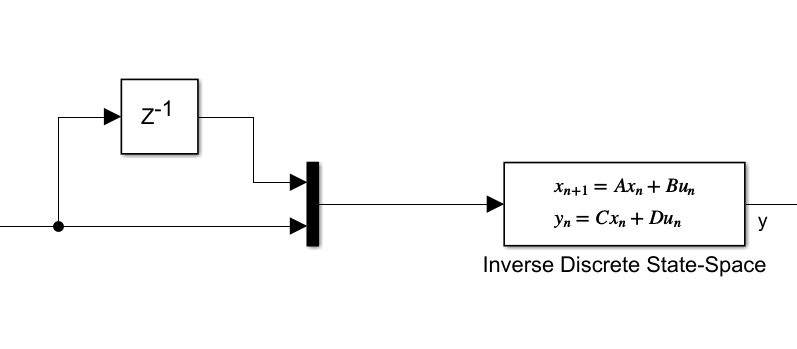
\includegraphics[scale=0.5]{graphics/inverseSS}
\caption{The inverted state space model with the a one time-step input delay.}
\label{fig:inverseSS}
\end{figure}

This results in a robust inverse system. When used in the IMC loop it is able to perfectly track simple sinusoid input at a one time-step delay. This delay is negligible for sufficiently small time-steps.

\section{Adaptive law}
\label{adaptiveLawSection}
%Figure of Ringwood's Control system somewhere?
Ringwood's paper\cite{ringwood} on Simple and Effective control makes use of an adaptive filter described as 
$\frac{1}{H(t)}$.  This filter takes the dominant frequency and amplitude of the incoming wave excitation force($F_{ex}$) and outputs a reference velocity($v_{ref}$). The control system then makes the float track this reference velocity as accurately as possible.

Ringwood has shown through extensive study that maximum energy extraction in 1DOF occurs when the float oscillation is in phase with the excitation force's dominant frequency\cite{ringwood}. So to realise maximum energy extraction, ``The velocity should always be in phase with the excitation force and it should have an amplitude that is modulated in the frequency-domain by the inverse of double the radiation resistance $\frac{1}{2B(\omega)}$''\cite{ringwood}.

This is expanded to cover the two controlled dimensions of the float: Surge and Heave. It is assumed that maximum power extraction may be achieved in both dimensions as they are independent. For example, uneven excitation in these two dimensions will result in elliptical motion of the float.

To construct the filter the radiation response of the float in each dimension must be modelled. The radiation response refers to the forces on the float due to the waves that are generated by the float's motion, and which then carry energy away from the system. These responses can be modelled by transfer functions. The project supervisor has provided these transfer functions and they are shown in appendix \ref{radiationTFs}.

These functions transfer float velocity to radiation force. We need to find the amplitude of the radiation response at a given frequency. Bode plots relate the amplitudes and frequencies of systems. Figure \ref{bodePlots} shows bode plots of both functions.

\begin{figure}
\centering
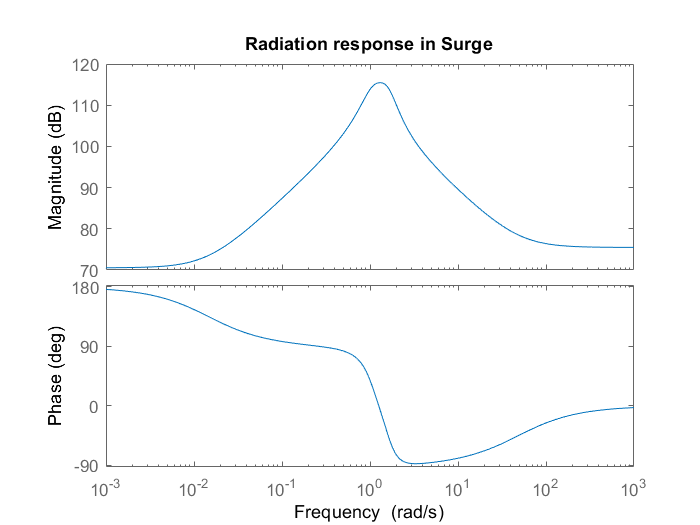
\includegraphics[scale=0.5]{graphs/radiationBodeSurge}
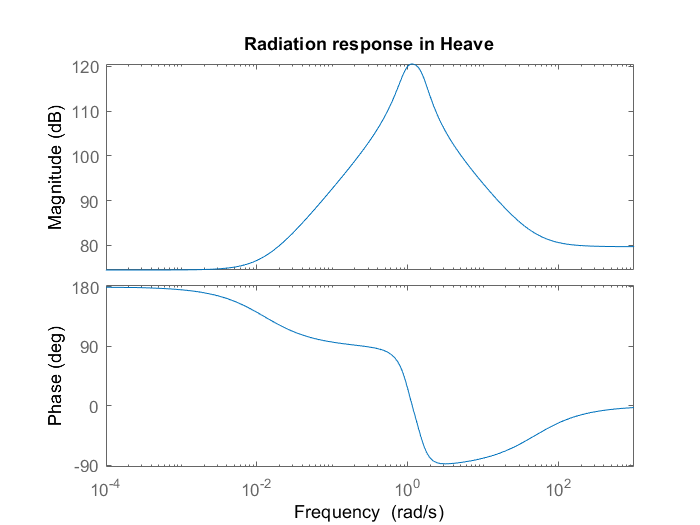
\includegraphics[scale=0.5]{graphs/radiationBodeHeave}
\caption{Bode plots of the Surge and Heave radiation force transfer functions. Created using the MATLAB bode command.	}
\label{bodePlots}
\end{figure} 
\FloatBarrier

The data from these plots is then turned into lookup tables to be used in the filter as shown in the code in appendix \ref{inputFile}. Given the dominant frequency of $F_{ex}$ the radiation amplitude response can be obtained using the lookup table block in Simulink as shown in figure \ref{adaptiveLawSimulink}. According to Ringwood\cite{ringwood} the velocity reference may be obtained via the relation,

\[
v_{ref}(t)=\frac{1}{2B(\hat{\omega})}f_{ex}(t)
\]

where $\hat{\omega}$ is the radiation force amplitude response produced by the dominant frequency. This is implemented as shown in figure \ref{adaptiveLawSimulink}. Hence $v_{ref}$ is obtained and given as an output.
 
\begin{figure}
\centering
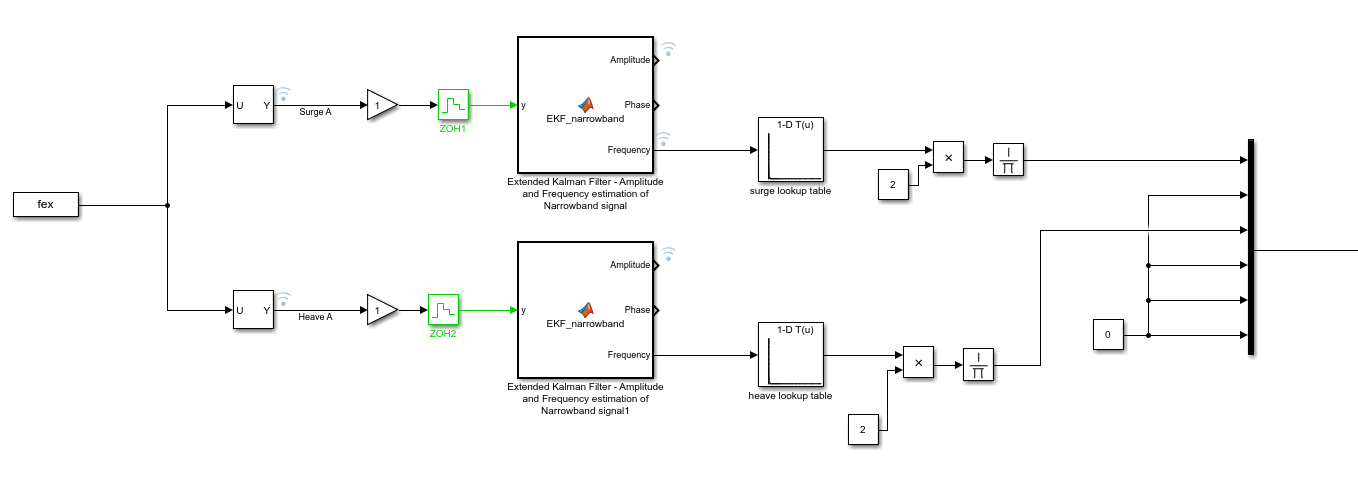
\includegraphics[scale=0.5]{graphics/adaptiveLaw}
\caption{The fully implemented adaptive filter in the Simulink environment.}
\label{adaptiveLawSimulink}
\end{figure} 

\FloatBarrier
\section{Filtering Wave Excitation Force}
\label{EKF}
It is necessary to make an estimate of the frequency of $F_{ex}$ in order to produce $v_{ref}$ as described in section 
\ref{adaptiveLawSection}. An extended kalman filter is used to extract these parameters from $F_{ex}$. The programming of the extended kalman filter block was provided by the project supervisor, and the tuning of it was performed by the author. A copy of the block's code with the tuning parameters used is provided in appendix \ref{EKFCode}

Kalman filters are commonly used in systems where physical processes are well modelled. Physical measurements and predictions are combined in an iterative process to produce more accurate readings than could otherwise be achieved in real time. It relies on data from both processes being normally distributed so that they can be combined simply.

The EKF used in this project is developed from the EKF described by Fusco, F. in his PhD thesis "Real-time Forecasting and Control for Oscillating Wave Energy Devices"\cite{EKF}. Figure \ref{kalmanAmplitudeEnvelope} shows the filter's estimation of the wave amplitude. Figure \ref{kalmanFrequency} shows its estimation of the frequency of a sinusoidal wave of frequency 0.1 rad/s.

\begin{figure}
\centering
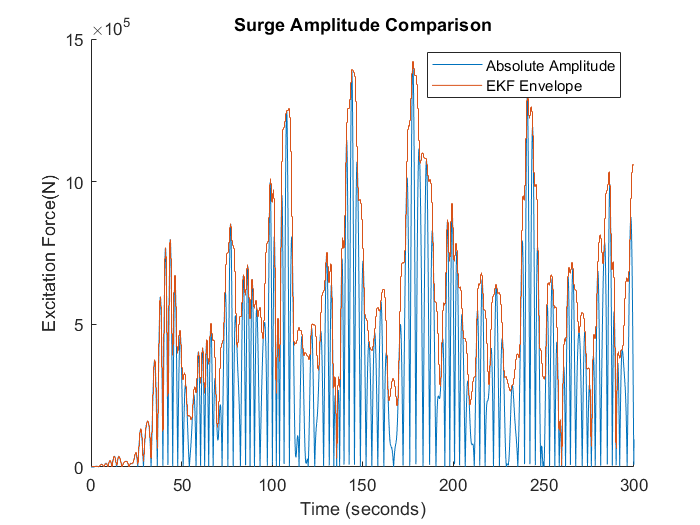
\includegraphics[scale=0.5]{graphs/EKFSurgeEnvelope}
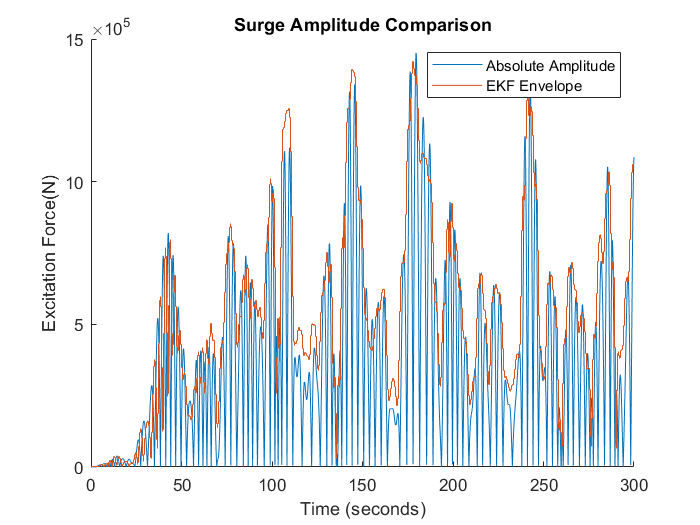
\includegraphics[scale=0.5]{graphs/EKFHeaveEnvelope}
\caption{Graphs showing the Amplitude Envelope of the EKF compared to the absolute amplitude of the wave excitation force.}
\label{kalmanAmplitudeEnvelope}
\end{figure} 

\begin{figure}
\centering
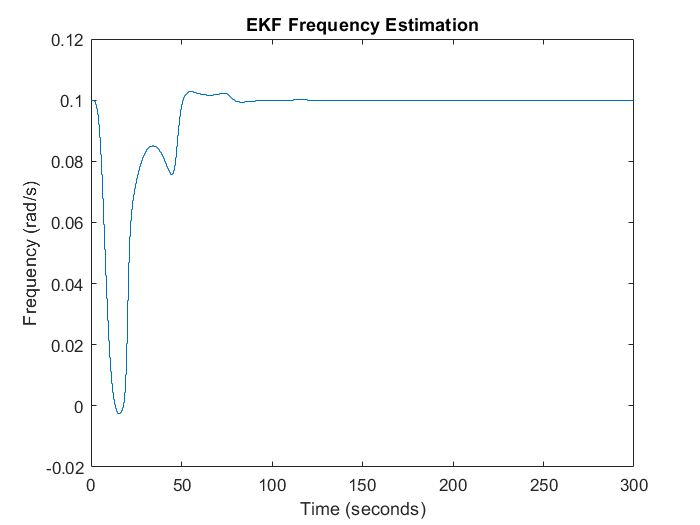
\includegraphics[scale=0.5]{graphs/EKFfrequency}
\caption{Graph showing the EKF estimation of wave frequency. The input is a sinusoid of frequency 0.1 rad/s.}
\label{kalmanFrequency}
\end{figure} 

The estimation of frequency takes more time to reach the correct value than desired. This may have an impact on energy extraction and system stability.

\section{Constraints Handling}
\label{constraintsHandlingSection}
The control strategy has so far only focused on tracking the best velocity for energy capture. There are also physical constraints which must be considered. Motions in all of the non-controlled dimensions are already very small and  need not be specifically controlled. In the controlled dimensions of heave and surge there are large amplitude motions which may exceed the physical limits of the device.

For the WaveSub device the physical limits in heave and surge are $\pm 5m$ from the home position. A limit of $\pm 3m$ is imposed in the surge dimension as a safety factor. It is important that the float does not crash into the platform.

Ringwood \cite{ringwood} proposes a method to limit the amplitude of the reference velocity, which prevents the float from deviating outside of physical limits so long as the mean of the float's velocity is zero and there is good tracking of the reference velocity. As shown in the results in chapter \ref{results} this is not necessarily the case.

To impose this limit a new term is calculated which can be expressed as, 

\[
\frac{\hat{\omega}X_{lim}}{\hat{A}}
\]

where $\hat{\omega}$ is the frequency of $F_{ex}$; $\hat{A}$ is the amplitude of $F_{ex}$ in metres; and $X_{lim}$ is the physical limit in the relevant dimension in metres.

The adaptive law from section \ref{adaptiveLawSection} is then modified with conditional logic such that,

\[
\frac{1}{H(t)} = 
\left\{\begin{matrix*}[l]
\frac{1}{2B(\hat{\omega}}, \textup{ if } \frac{\hat{\omega}X_{lim}}{\hat{A}}>\frac{1}{2B(\hat{\omega})}\\
\frac{\hat{\omega}X_{lim}}{\hat{A}}, \textup{ otherwise.}\\
\end{matrix*}\right.
\]

Figure \ref{velocityConstraints} shows how this logic was implemented in Simulink.
\FloatBarrier
\begin{figure}

\centering
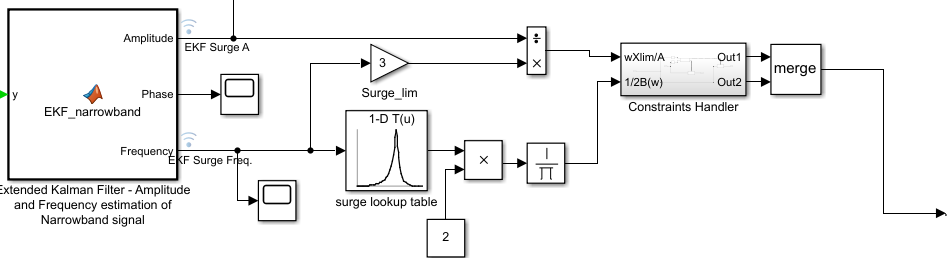
\includegraphics[scale=0.5]{graphics/constraintsTop}
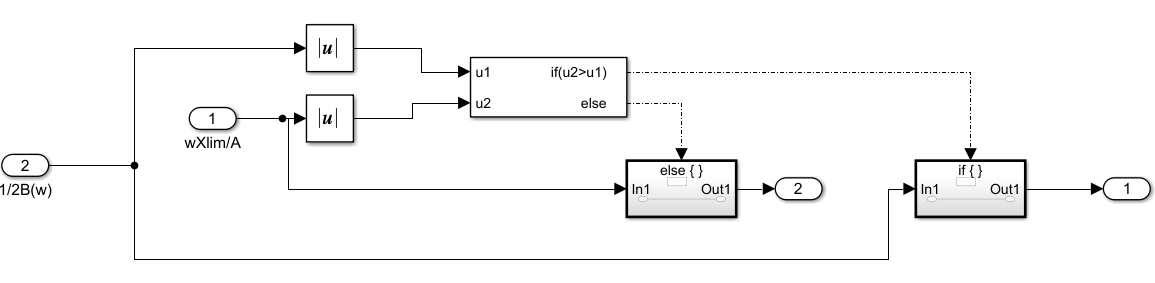
\includegraphics[scale=0.5]{graphics/constraintsBottom}
\caption{Integration with adaptive law(top) and `Constraints handler' subsystem implementation(bottom).}
\label{velocityConstraints}
\end{figure}

\FloatBarrier
\section{Integral feedback}

Implementation of the prior sections of this chapter is all that is needed to fully realise Ringwood's Simple and Effective control. However, as shown in the results in chapter \ref{results} this results in a drift that quickly violates physical constraints. This drift may arise due to the fact that the mean of the float's velocity is non-zero. This would mean that limiting the amplitude of the velocity as described in section \ref{constraintsHandlingSection} is insufficient.

Introducing an integral feedback loop was investigated as a possible solution. There are many ways to implement this. Figure \ref{integralFeedbackLoop} shows one. There are two summing junctions in the figure. Routing the integral feedback path to either one produces a different implementation. There is also a decision to made on whether to use the first or second integral of Velocity. 

\begin{figure}
\centering
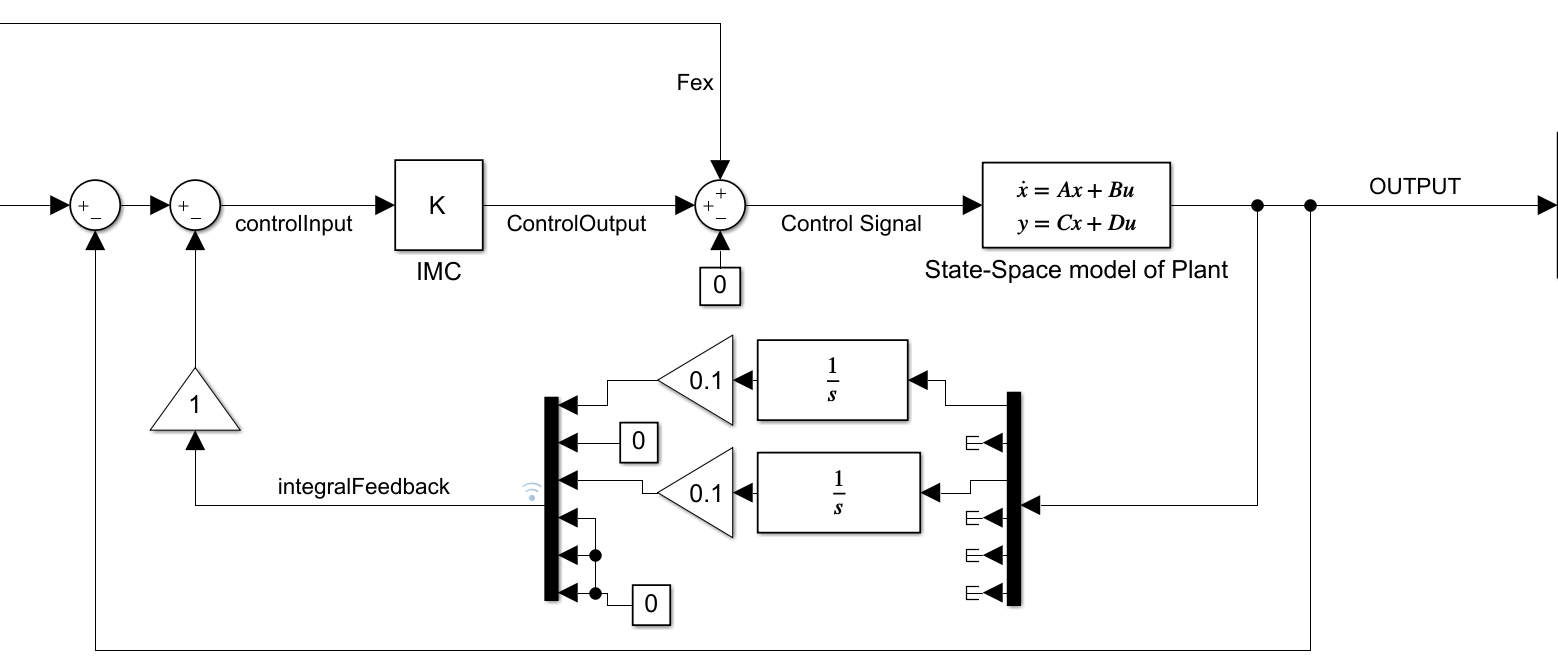
\includegraphics[scale=0.5]{graphics/integralFeedback}
\caption{One implementation of the integral feedback loop.}
\label{integralFeedbackLoop}
\end{figure}

In this project it was found that the implementation as shown in figure \ref{integralFeedbackLoop} produced better power results and better managed the physical constraints.

The gain was tuned with the constraints turned off. It keeps the mean of the velocity to within $0.1ms^{-1}$ of 0. Ringwood's constraints can then be used to limit the velocity, and therefore the position, as intended.

\chapter{Results}
\label{results}

All simulations presented here have been created using wave data generated by WecSim according to the Pierson-Moskowitz spectrum relation \cite{OGPM} with a sampling rate of $\frac{1}{0.02s}=50Hz$.

The sea states that have been simulated are a combination of two ranges. The range of significant sea heights($H_s$) is from 0.5 to 6.5 metres in increments of 0.5m. The range of wave periods($T_e$) is from 6 to 16 seconds in increments of 1 second. According to Hillis \cite{andyMPC} this is representative of the sea states likely to be encountered by the WEC.


\section{Tracking Performance}
The tracking performance is near ideal save for a delay of one time-step due to the use of the state-space model as the plant. Figure \ref{SSTracking} shows a typical example of this tracking of reference velocity.

\begin{figure}
\centering
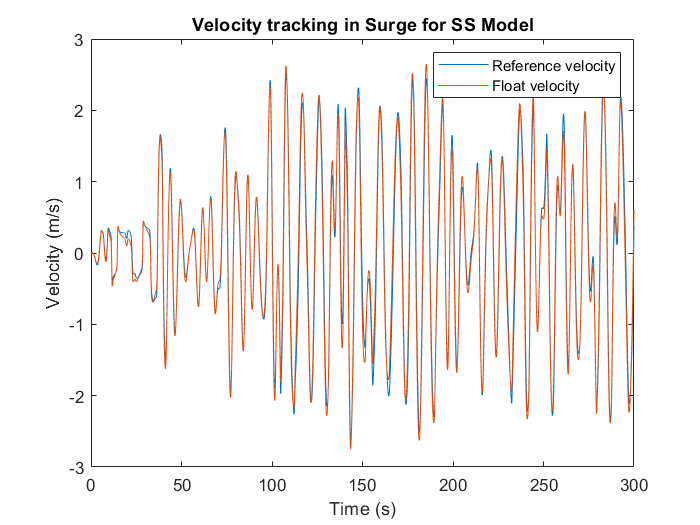
\includegraphics[scale=0.5]{graphs/SS_surgeTracking}
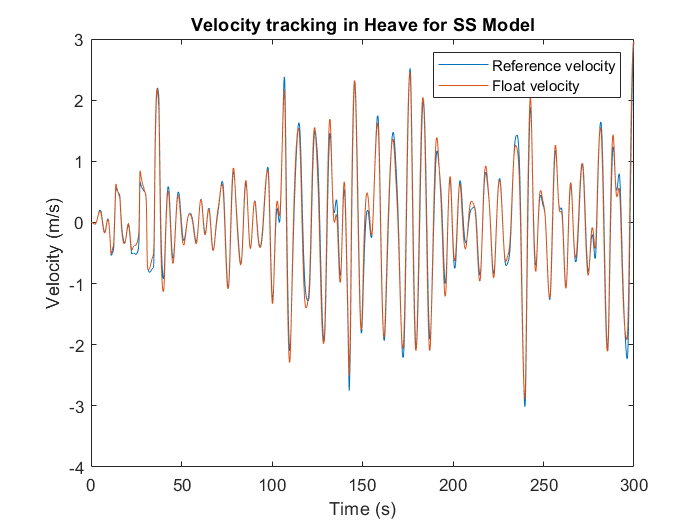
\includegraphics[scale=0.5]{graphs/SS_heaveTracking}
\caption{Tracking performance of the IMC with the State Space Model as the plant. Hs = 3, Te = 10.}
\label{SSTracking}
\end{figure} 

Unfortunately this tracking performance does not carry into wecSim. Figure \ref{wecSimTracking} superimposes the float velocity in surge and heave on the reference velocity. The frequencies are identical, but the amplitude of the float velocity is much larger than of the reference velocity.

\begin{figure}
\centering
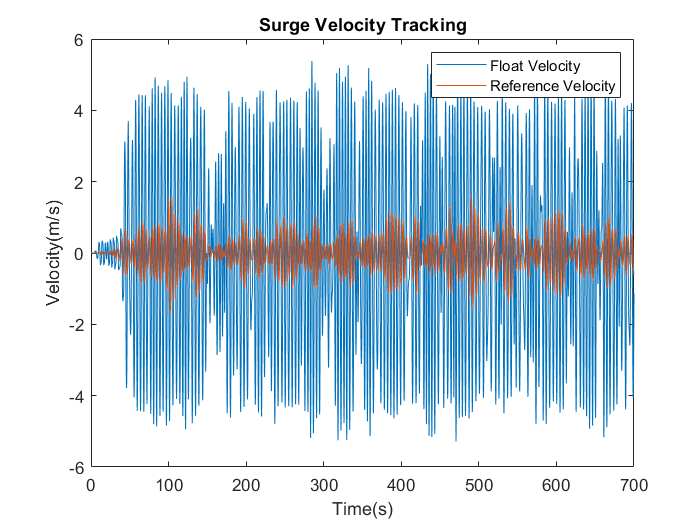
\includegraphics[scale=0.5]{graphs/wecSimSurgeTracking}
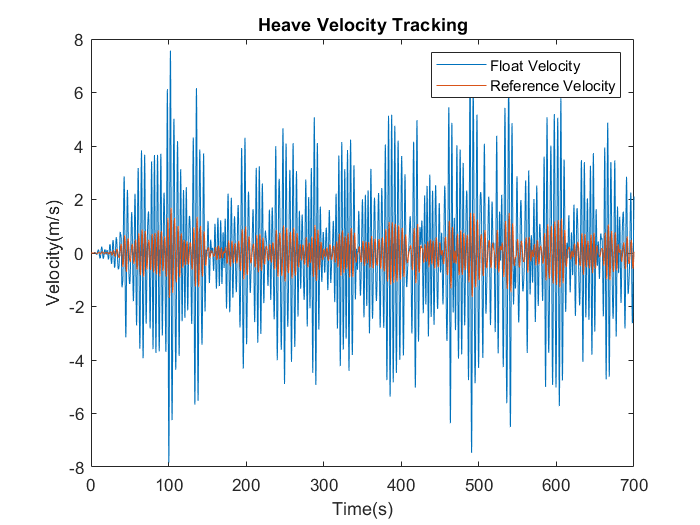
\includegraphics[scale=0.5]{graphs/wecSimHeaveTracking}
\caption{Tracking performance of the float in the wecSim environment.}
\label{wecSimTracking}
\end{figure} 

\FloatBarrier
\section{Power output using State-Space model}
The power generated using the Simple and Effective control system is compared against the power generated by an optimally tuned passively damped system as described in ``Active control for multi-degree-of-freedom wave energy converters with load limiting'' \cite{andyMPC}.

This passive-damping system relies only on a damping co-efficient that relates cable velocity to cable tension. i.e.,

\[
\textup{Cable Tension} = \textup{Cable Velocity} \times \textup{Damping Co-efficient}
\]

in the axis of each cable. The co-efficient is optimally chosen for each wave period. This could feasibly be performed in reality using an adaptive law and a method of measuring the sea-wave frequency such as the EKF method described in section \ref{EKF}.

Table \ref{passiveResults} shows the mean power generated in each sea state by the passively damped system. This table is reproduced from unpublished work by A. Hillis \cite{andyMPC}.

\begin{table}
\hspace{-3cm}
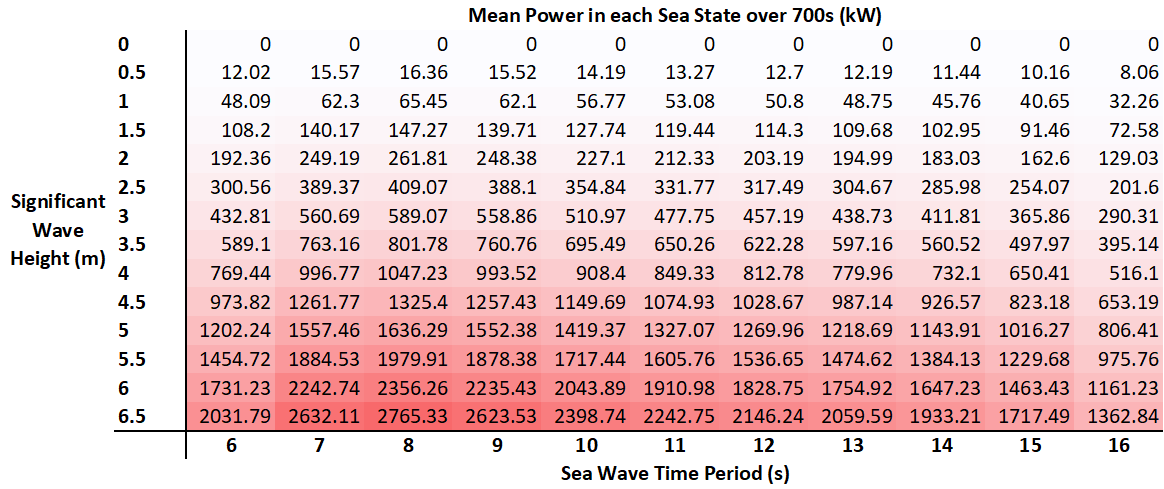
\includegraphics[scale=0.7]{tables/passiveResults}
\caption{Power generated by optimally tuned passive damping. Reproduced from\cite{andyMPC}.}
\label{passiveResults}
\end{table}
\FloatBarrier

Tables \ref{SAEResults} and \ref{SAEPercents} show the mean power generated by the Simple and Effective Control Strategy without an integral feedback loop. Whilst this control strategy does generate power, it does not comply with physical system constraints. Table \ref{SaEPosition} shows the maximum heave and surge displacements with those beyond physical limits highlighted.

Power is calculated as the product of the control force output of the IMC controller and the resultant float velocity. The mean power is then calculated as the arithmetic mean of the power produced over the 700 second sample time. Power generation is negative by convention. The arithmetic mean is used as opposed to the geometric mean as instantaneous power oscillates between positive and negative.

\begin{table}
\hspace{-3cm}
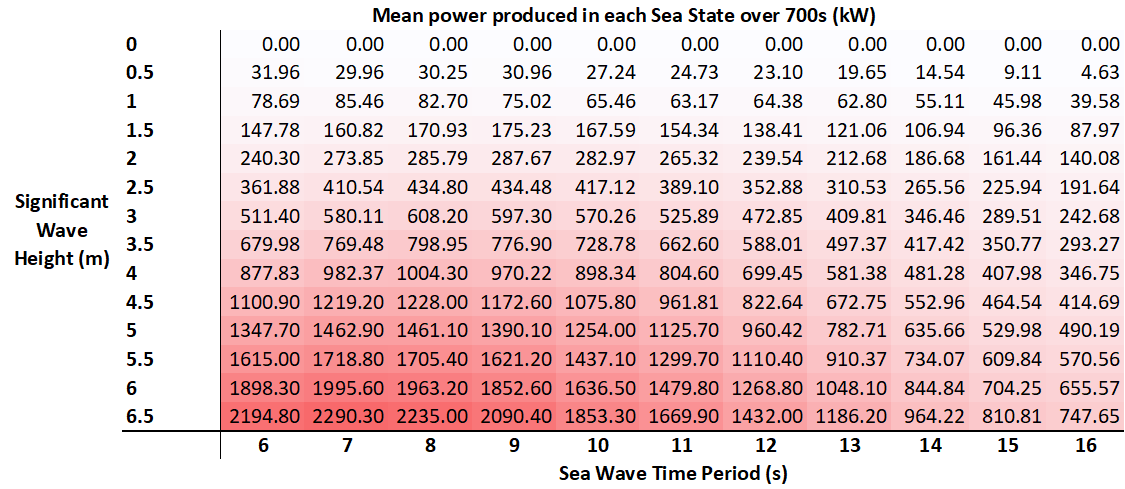
\includegraphics[scale=0.7]{tables/SaEResults}
\caption{Power generated by Simple and Effective control model. Darker red indicates higher power.}
\label{SAEResults}
\end{table}

\begin{table}
\hspace{-3cm}
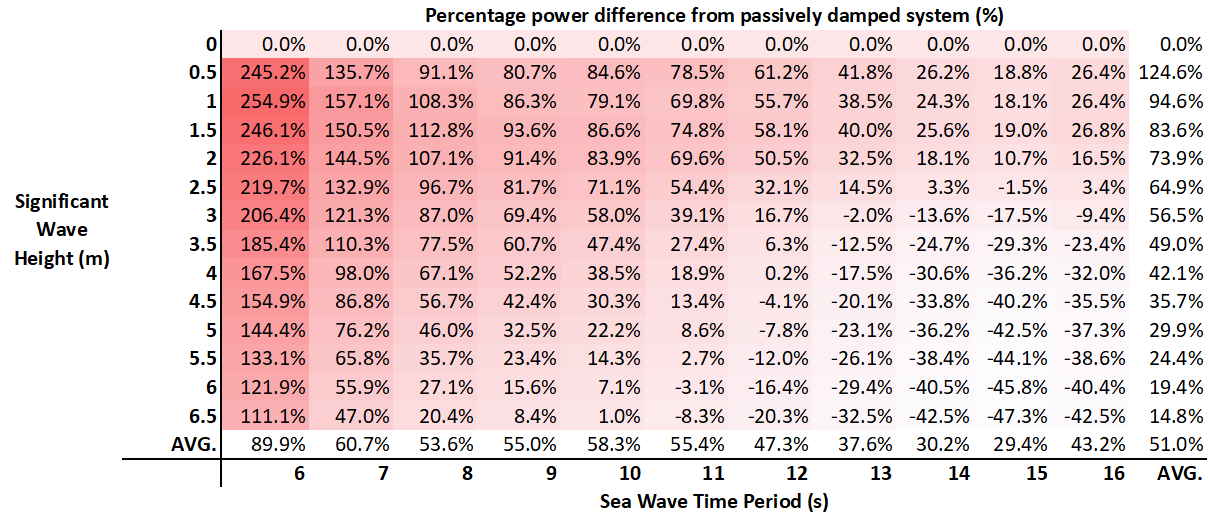
\includegraphics[scale=0.7]{tables/SaEPercent}
\caption{Percentage differnces in power generated by Simple and Effective control compared to passive damping. Darker red indicates higher difference. Averages have been excluded from this formatting.}
\label{SAEPercents}
\end{table}

\begin{table}
\centering
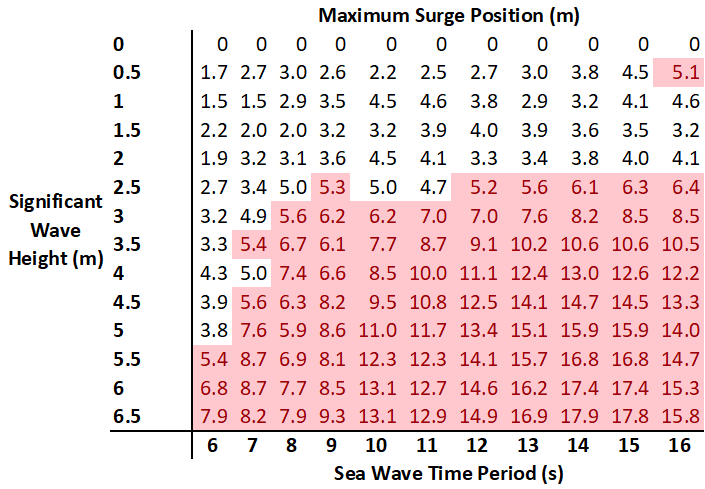
\includegraphics[scale=0.7]{tables/SaESurgePos}
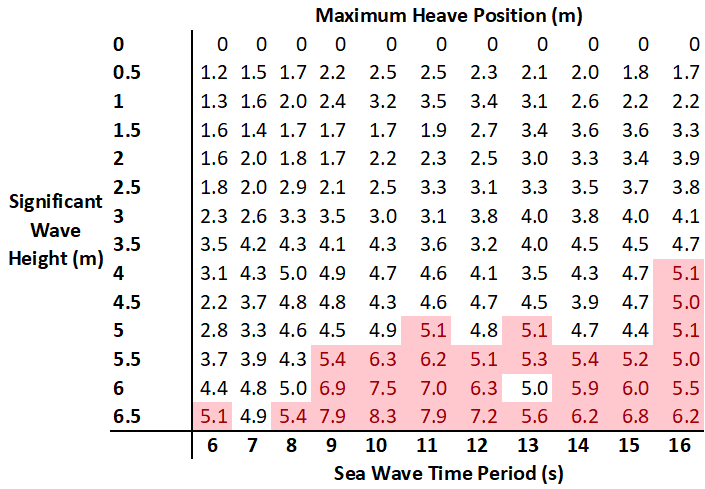
\includegraphics[scale=0.7]{tables/SaEHeavePos}
\caption{Tables showing maximum position deviation in heave and surge. Red indicates that physical constraints have been exceeded.}
\label{SAEPosition}
\end{table}

\FloatBarrier

With the addition of integral feedback control physical constraints are observed as shown in table \ref{integralPosition}. No significant effect on power generation is observed as shown in tables \ref{integralResults} and \ref{integralPercents}.


\begin{table}
\hspace{-3cm}
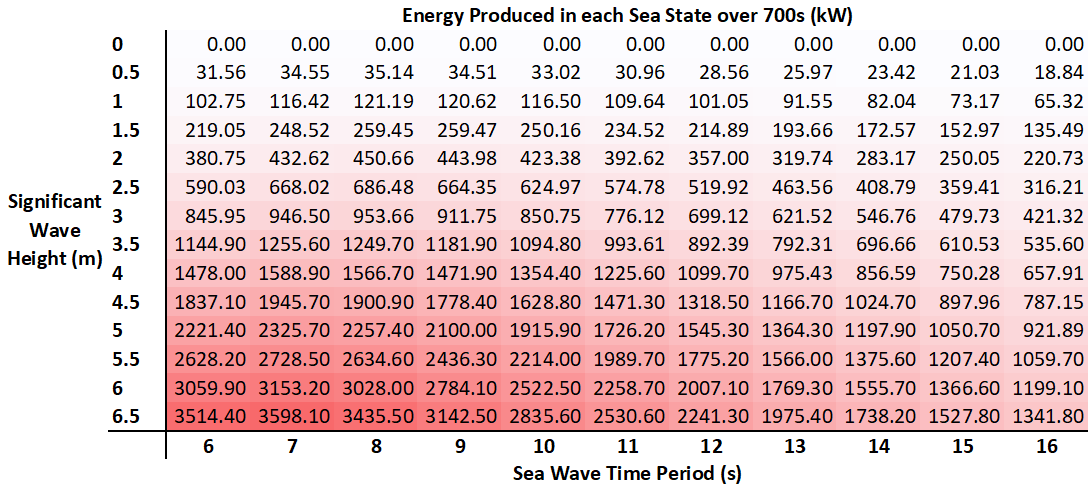
\includegraphics[scale=0.7]{tables/integralControlResults}
\caption{Power generated by integral feedback model. Darker red indicates higher power.}
\label{integralResults}
\end{table}

\begin{table}
\hspace{-3cm}
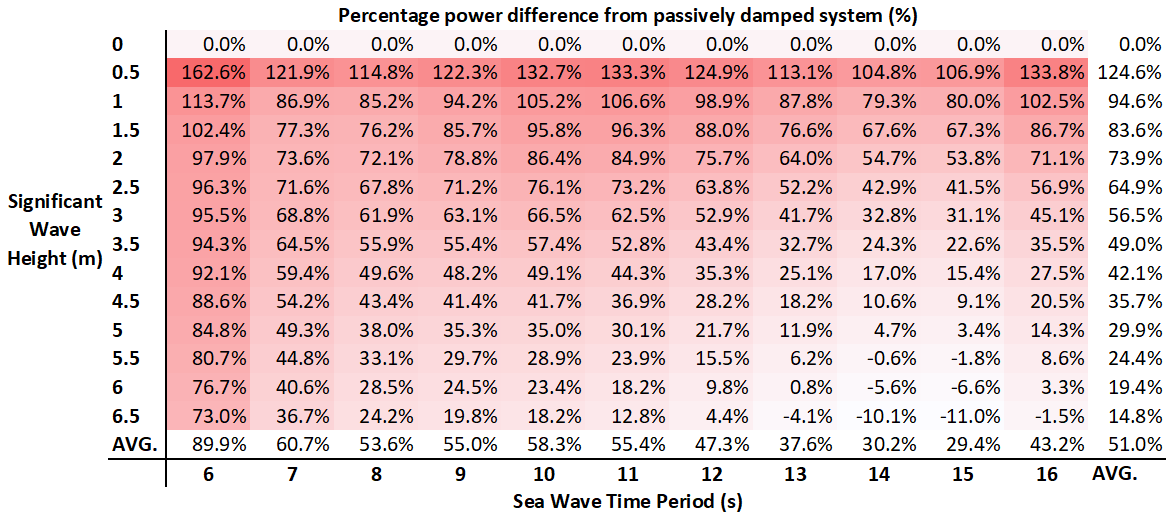
\includegraphics[scale=0.7]{tables/integralControlPercent}
\caption{Percentage differnce in power generated by Simple and Effective control with integral feedback compared to passive damping. Darker red indicates higher difference. Averages have been excluded from this formatting.}
\label{integralPercents}
\end{table}

\begin{table}
\centering
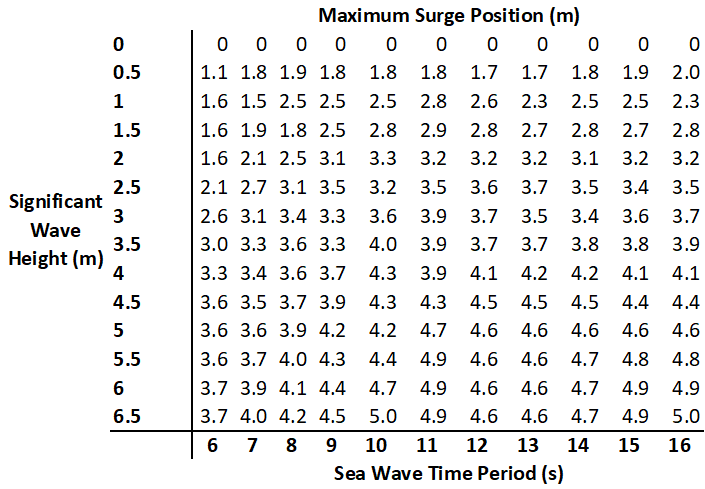
\includegraphics[scale=0.7]{tables/integralSurgePos}
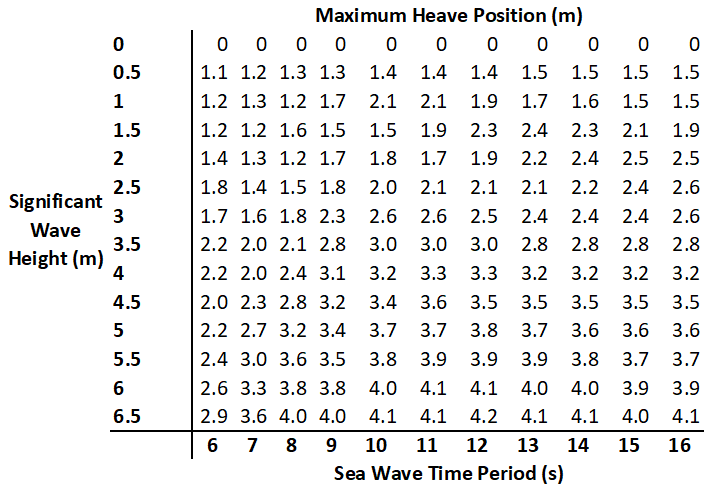
\includegraphics[scale=0.7]{tables/integralHeavePos}
\caption{Tables showing maximum position deviation in heave and surge for the integral feedback control model. Physical constraints were not exceeded in any case.}
\label{integralPosition}
\end{table}



\FloatBarrier
\section{Power output of wecSim model}
Due to difficulties discussed in section \ref{difficulties} the control system was only crudely implemented in the WecSim environment. Figure \ref{wecSimImplementation} shows this implementation.

\begin{figure}
\centering
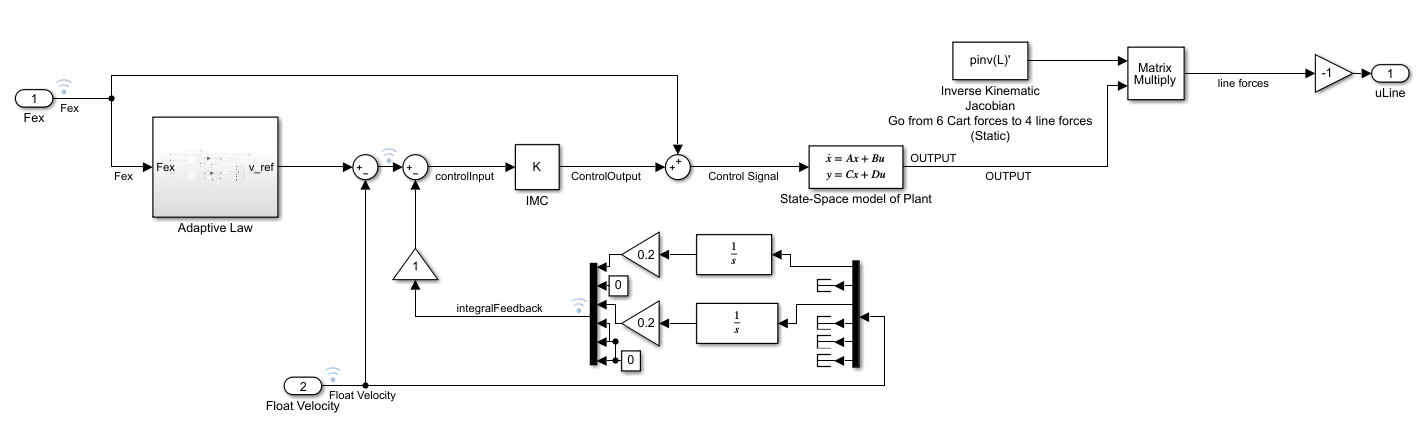
\includegraphics[scale=0.5]{graphics/wecSimImplementation}
\caption{The implementation of the integral feedback control system in the WecSim environment.}
\label{wecSimImplementation}
\end{figure} 

Some small amount of power was generated by the device despite the poor tracking shown in figure \ref{wecSimTracking}. Constraints were violated in many sea states due to the increased amplitude of the float velocity in surge.

\begin{table}
\centering
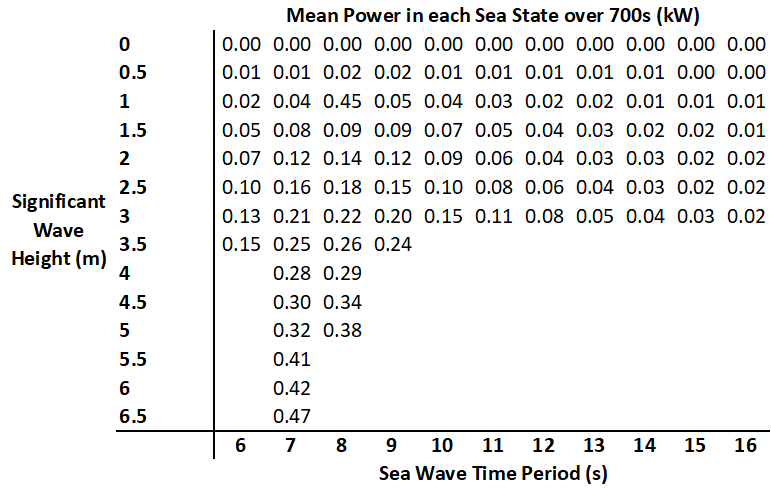
\includegraphics[scale=0.7]{tables/wecSimResults}
\caption{Table showing mean power produced by the crude WecSim implementation. Missing values are due to constraints violation.}
\label{integralPosition}
\end{table}

\chapter{Discussion}

In place of the WecSim environment, the state-space model used for development of the IMC was used to produce most results. This is undesirable since it makes more assumptions than the WecSim environment, and is identical to the model used in the IMC. The highly accurate tracking produced using this model is therefore unsurprising.

When implemented in the WecSim environment the tracking is worse. As shown in figure \ref{wecSimTracking} whilst the frequency of the floats' velocity matches that of the reference signal its amplitude does not. It appears by simple inspection that the amplitudes may be proportional, but this has not been properly investigated due to the constraints discussed below in section \ref{difficulties}.

One potential explanation for this amplitude difference is that the amplitude response of the controller at high frequencies is large. Figure \ref{IMCBode} shows the surge-surge and heave-heave responses of the IMC controller. The tested range of sea wave frequencies is between 0.4 rad/s ($Te = 16$) and 1 rad/s ($Te=6$). In this range the bode plot reveals that the amplitude response grows exponentially with frequency. This implies that the controller produces a large response to high frequency signals which may be inappropriate. These frequencies may be present in the WecSim environment but not the state-space model environment due to WecSim's modelling of high frequency responses such as radiation forces. This problem could possibly be resolved with the use of a high-pass filter. One possible expression of this filter is as a transfer function,

\[
\frac{\textup{Output}}{\textup{Input}}=\frac{s}{s+2\pi}
\]

where $2\pi$ is the cut-off frequency. This corresponds to 1 Hz which is the upper bound on typical sea-wave frequencies \cite{PMReview}.

Another potential explanation is that the Massay-Sain IMC features a real-time delay where Dr. Hillis' system does not. When transforming to the frequency domain a real-time delay becomes an exponential term. For example, if a function $f(t)$ is shifted by time $a$,
\[
\mathcal{L}[u(t-a)f(t-a)]=e^{-as}F(s)
\].
This exponential term could be responsible for the large amplitude response.

Signal properties that are present in WecSim but not the State-Space model environment are examples of model error.  It was hoped that this model error would be insignificant as detailed in section \ref{section:assumptions}. This was mistaken. This implies that this implementation of Simple and Effective control is not robust to model error.



\begin{figure}
\centering
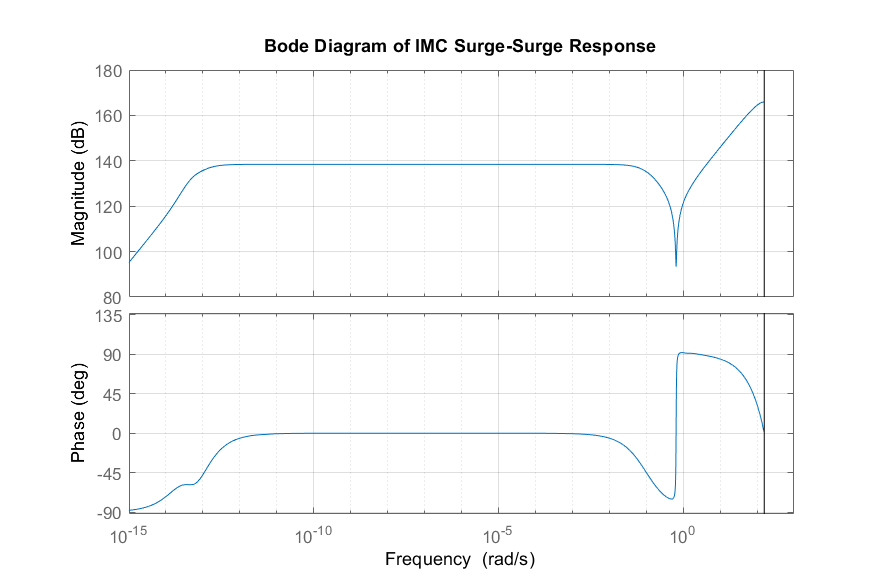
\includegraphics[scale=0.5]{graphs/IMCBodeSurge}
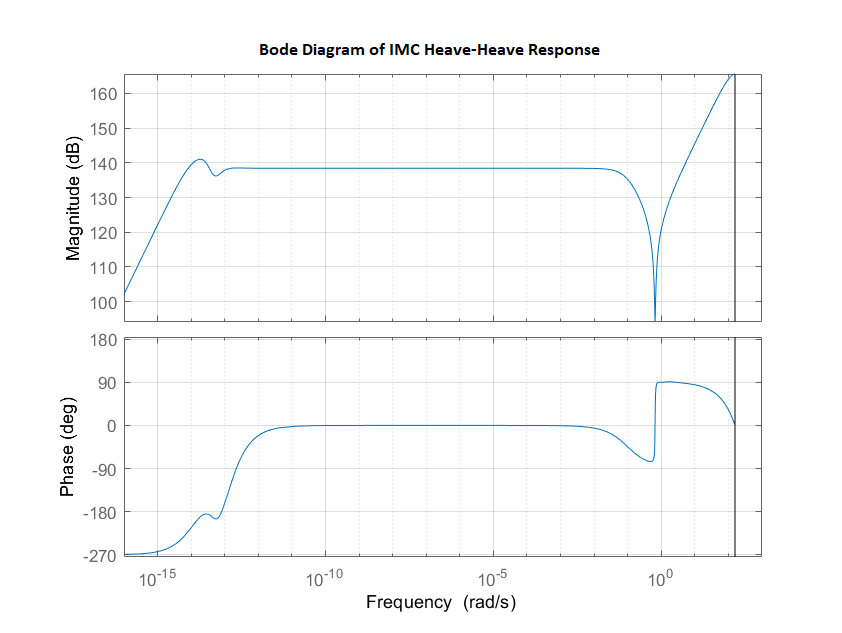
\includegraphics[scale=0.5]{graphs/IMCBodeHeave}
\caption{Bode plots showing the surge-surge(top) and heave-heave(bottom) responses of the IMC controller.}
\label{IMCBode}
\end{figure} 

\FloatBarrier
\section{Suitability for review}
Overall it has been demonstrated that the Massay-Sain inverse State-Space model is robust for practical purposes. It was stable for all tested sea-states in both environments. Whilst the controller's response in the WecSim environment is too large, it is still finite.

Whilst imperfect, this implementation of the IMC is suitable for the purposes of review. It is robust and produces good tracking whilst being distinct from the IMC developed by A. Hillis, which uses transfer function approximations.

By extension the entire implementation of Simple and Effective Control is suitable for review. It is a reproduction of the same methodology described by Ringwood \cite{ringwood} which produces realistic results. Further it has the IMC and an independent Simulink implementation as meaningful distinctions from previous work. The one area in which work has been re-used is the implementation of the Extended Kalman Filter. This filter-is well understood but the potential remains for the re-production of errors. Future work should consider the filter for investigation.


\section{Difficulties with the WecSim environment}
\label{difficulties}
Despite the author's best efforts the control system was not realised in the wecSim environment until the end of the project time frame. The issues with the environment arose from version differences between MATLAB version R2017b and R2018b. Most importantly, R2018b does not automatically update the cache file of the simulink model automatically, meaning that changes to the model do not take effect. This does not appear to be the case in R2017b, where the project supervisor's work was developed.

This issue was resolved by either manually or programmatically deleting the cache file between every simulation run to force an update. Future work should ideally find a way to restore the automatic cache-updating process.

Further versioning issues include changes to the syntax for the legend() command, and the incompatibility of the bemIO environment. Fixes for these issues are included in the project source code.

\section{Existence of the drift problem}

It is clear from table \ref{SAEPosition} that the Simple and Effective controller does not keep the float within physical constraints for most of the sea states tested. It is not clear from the table what the behaviour of the float looks like when it violates these constraints. Figure \ref{constraintBreaking} shows an example from one case in which constraints were violated. The values for the positions are taken as the integral of the float's velocity with respect to time.

\begin{figure}
\centering
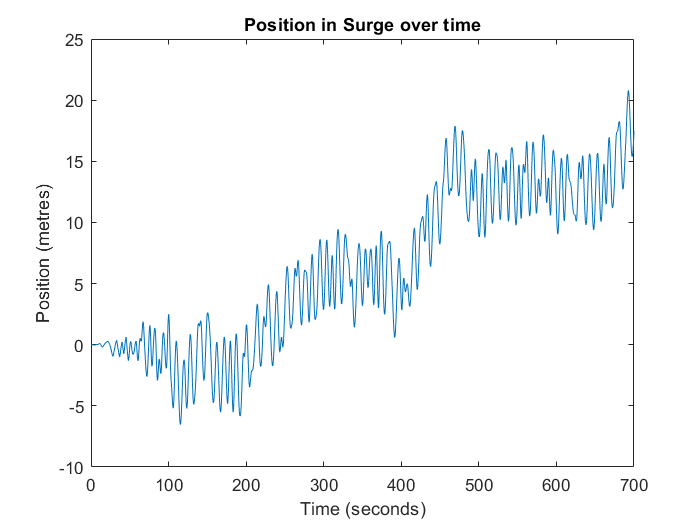
\includegraphics[scale=0.5]{graphs/constraintBreakingSurge}
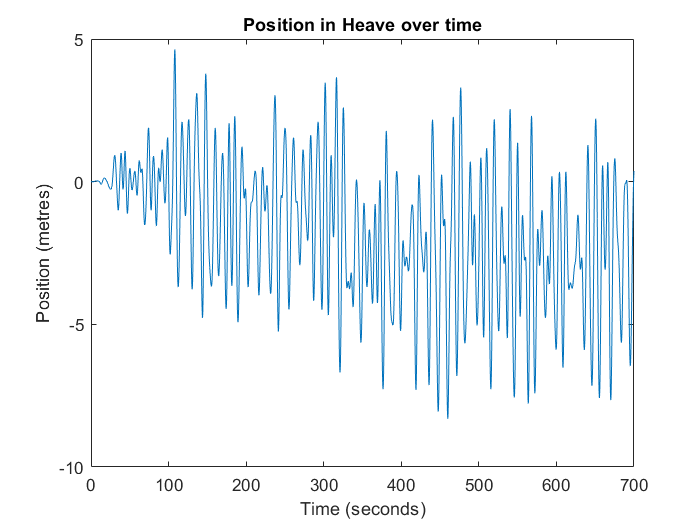
\includegraphics[scale=0.5]{graphs/constraintBreakingHeave}
\caption{Graphs showing the position of the float in Surge (top) and Heave (bottom) during a simulation run. The input data was a sea-state with $H_s = 3$ and $T_e = 10$}
\label{constraintBreaking}
\end{figure} 

In both dimensions the amplitude of the oscillations is limited according to the method Ringwood proposed \cite{ringwood}. However, the mean of the oscillation is not constant in either case. In surge especially the mean drifts positive, occasionally staying at what appear to be new set-points. In the case of Heave the mean drifts negative, and more slowly. This drift behaviour is observed in all other tested sea states. It is not necessarily positive or negative and may change over the course of a single run.

Due to the simplistic nature of the State-Space model based simulation, and its distinctiveness from prior work, this is strong evidence for the existence of the drift problem.

\FloatBarrier
\section{Correcting Drift}
The drift is caused by the fact that the integral of the velocity with respect to time has a non-zero average for short periods. This may be caused by the sea-state parameters changing over time, which causes a transition period for the system. In any case, the constraints proposed by ringwood are not sufficient to prevent this drift.

A hypothesis was proposed that the drift could be corrected with minimal impact on power generation using a small integral term. This term drives the mean of the float's velocity to 0, and by extension the mean of its position. Ringwood's constraint method could then be relied on to limit amplitude of the float's oscillation.

This hypothesis was tested using the implementation shown in figure \ref{integralFeedbackLoop}, and produced the results shown in tables \ref{integralResults} and \ref{integralPercents}.

Physical constraints were not exceeded for any of the tested sea-states. The power generation has been positively affected in more violent sea states and reduced in gentler ones. The power gain in violent sea-states was an unintended result. The average mean power generated across all states was not significantly affected. Power gains in violent sea-states compensated for power lost in gentle sea-states.

Power may have been gained in gentler sea-states due to overshoot produced by the integral term. This would contradict Ringwood's assertion\cite{ringwood} that Simple and Effective control produces near-maximal power generation.

The unintended result and the simplicity of the model reduce the trust that should be put in these results. The hypothesis could not be refuted. This implies weak evidence that the drift problem can be rectified using this method.

\FloatBarrier
\section{Power Generation}
Overall the results show that Simple and Effective control was able to produce more power than a passively damped, optimally tuned system in a majority of sea-states. It is also able to enforce physical constraints where the passive system might violate them due to a lack of control.

Power generation gains were most improved in gentle sea-states. Power generation improvements decreased as wave height and period increased, eventually generating less power than the passive system.

The average mean power improvement across all sea-states was 51\%. This figure is not as applicable as it may appear. In reality some sea-states are more common. This combined with the fact that power gain was improved for some sea-states and made worse for others means that any amount of power gain or loss over the passive model may be produced given different distributions of sea-states.

The WecSim implementation showed that even when the tracking performance was poor, some small amount of power was produced albeit much less than in the passive model.

\chapter{Conclusions}
In this work the Simple and Effective control strategy proposed by Fusco and Ringwood\cite{ringwood} was adapted for a 6DOF WEC. The produced model was distinct from prior work by the project supervisor A.Hillis, making it useful for review. In particular the novel application of the Massay-Sain inverse algorithm has produced a robust inverse model of the WEC that is worth further study.

Due to difficulties with the WecSim simulation environment the state-space model originally used for development of the IMC was also used to model the WEC plant. This reduced the amount of the trust that can be assigned to positive results produced by this project. A crude version of the control system was eventually produced, and was found to have poor tracking performance whilst still generating a small amount of power. This suggests that the system's power production is not robust to model error, but that its stability is.

The first research question was whether the drift problem established by A. Hillis in prior work could be reproduced in an independently constructed model. It can.

The second research question was whether the drift issue could be resolved. Weak evidence was produced that it can be resolved using an integral feedback loop.

The final research question was how much power can be produced by this control strategy compared to a passively damped, optimally tuned system. It was shown that power production improvement of up to 162.2\% is possible in gentle sea-states, but that power production is made worse during violent sea-states to keep the float within physical constraints. The worst power production loss over the passively damped system was -11.0\%.

\section{Future Work}

Any future work using the Massay-Sain inverse method in this field should investigate its robustness against model error. This should be achieved within the WecSim environment or another well-established simulation environment.

The WecSim model produced in this project could be further developed to see if the presented results are still valid when fewer simplifying assumptions are made.

Alternative methods of correcting the float's position drift could be investigated. There is only weak evidence that the presented integral feedback loop is effective. There is a lack of theory to explain the effects that the loop had on the power generation of the system.


\bibliography{bibliography}
\bibliographystyle{IEEEtran}

\appendix
\appendixpage
\addappheadtotoc
\chapter{Radiation force Transfer Functions}
\label{radiationTFs}

\chapter{Project code: inputFile.m}
\label{inputFile}

\chapter{EKF Code}
\label{EKFCode}

\chapter{Github Link}
\label{github}


\end{document}